\documentclass[aspectratio=169,11pt]{beamer}
\usetheme{Boadilla}
\usecolortheme{seahorse}
\usepackage[T2A]{fontenc}
\usepackage[utf8]{inputenc}
\usepackage[english,russian]{babel}
\usepackage{booktabs}
\usepackage{graphicx}
\usepackage{amsmath}
\usepackage{xcolor}
\setbeamertemplate{navigation symbols}{}
\graphicspath{{figures/}}

\title[Implicit signals \& the RLHF axis]{Implicit signals and the activation space of preferences}
\subtitle{Subliminal transfer, persona vectors, and the RLHF axis}
\author{Олег Курилов}
\date{Июнь 2026}

\begin{document}

\begin{frame}\titlepage\end{frame}

% --- 2. Вопрос ---
\begin{frame}{Вопрос и три линзы}
Как неявные сигналы (данные дообучения, RLHF, activation steering) сдвигают «ценности» модели, и видно ли этот сдвиг внутри сети?

\vspace{0.6em}
Три линзы:
\begin{itemize}
  \item \textbf{Subliminal transfer.} Учитель со скрытым предпочтением выдаёт чистые числовые последовательности; ученик, дообученный только на этих числах, наследует предпочтение. В данных нет ни слова про сам объект.
  \item \textbf{Persona vectors в играх.} Направление черты прибавляется на слой, отвечающий за personality; поведение читается в экономических играх (Dictator, Trust, Ultimatum).
  \item \textbf{RLHF как persona vector.} $v_\text{RLHF}=\overline{h}(\text{Instruct})-\overline{h}(\text{base})$ на одинаковых промптах: его геометрия, поведенческий эффект и зависимость от extraction basis.
\end{itemize}
\vfill
{\footnotesize Модели: GPT-4.1-nano, Qwen2.5-7B, Qwen3-8B, Llama-3.1-8B. Судья: GPT-4.1-mini.}
\end{frame}

% --- 3. Главный вывод (тезис, один раз) ---
\begin{frame}{Главный вывод}
\begin{quote}
Видимый «рост альтруизма» от RLHF, измеренный LLM-судьёй, по большей части артефакт длины: instruct-модели отвечают длиннее, судья награждает длину. При вводе длины в регрессию ковариатой прирост падает до незначимого ($-0.44$ / $+0.09$, p=0.85 / 0.98).
\end{quote}
\vspace{0.4em}
Проще говоря: «RLHF сделал модель добрее» в основном означает, что она стала больше говорить, а судья читает многословие как доброту.
\vspace{0.5em}

{\footnotesize Доказательства — на слайдах про talk-vs-act и BERT. Более широкий тезис «измеренное выравнивание $\neq$ поведенческое» — это направление, а не итог: он держится на единственном поведенческом промпте (act-side, df$\approx$1).}
\end{frame}

% --- 4. Фаза I ---
\begin{frame}{Фаза I. Subliminal transfer (воспроизведение)}
Это известная работа (Cloud et al.\ 2025), воспроизведённая как фундамент: предпочтение можно перенести, ни разу его не назвав. Предпочтение оставляет измеримый след в активациях — отсюда и две следующие линзы.
\begin{table}\centering\footnotesize
\begin{tabular}{@{}llll@{}}
\toprule
Модель & Объект & База $\to$ Ученик & Режим \\
\midrule
GPT-4.1-nano & сова & 12.4\% $\to$ \textbf{56.7\%} & усиление (+44.3 пп) \\
Qwen 4B & кошка & 4.0\% $\to$ 10.2\% & усиление ($2.5\times$) \\
Qwen 0.8B & собака & 15.5\% $\to$ 12.9\% & защита от забывания \\
GPT-4.1-nano & кошка & 22.2\% $\to$ 22.9\% & нет эффекта \\
\bottomrule
\end{tabular}
\end{table}
\vspace{0.2em}
Скрытый сигнал линейно декодируется из активаций базовой модели с точностью \textbf{89.5\%} (5-fold; перестановочный $z={-}330$).
\end{frame}

% --- 5. Фаза II ---
\begin{frame}{Фаза II. Persona vectors в играх}
\begin{columns}[T]
\column{0.44\linewidth}
Черта живёт как направление. $c\cdot v$ прибавляется на слой, отвечающий за personality (L20); отдача в игре читается судьёй.
\begin{itemize}\footnotesize
  \item Sweep монотонный; базовая отдача в Dictator растёт примерно с \$17 до \$83.
  \item Разрыв по magnitude $\sim 2\times$ относительно статьи (L2-norm).
  \item При сильном steering coherence коллапсирует; рабочий диапазон $c\in[1,2]$.
  \item Крупнее модель — раньше коллапс: 8B теряет coherence при меньшем $|c|$, чем 7B.
\end{itemize}
\column{0.56\linewidth}
\centering
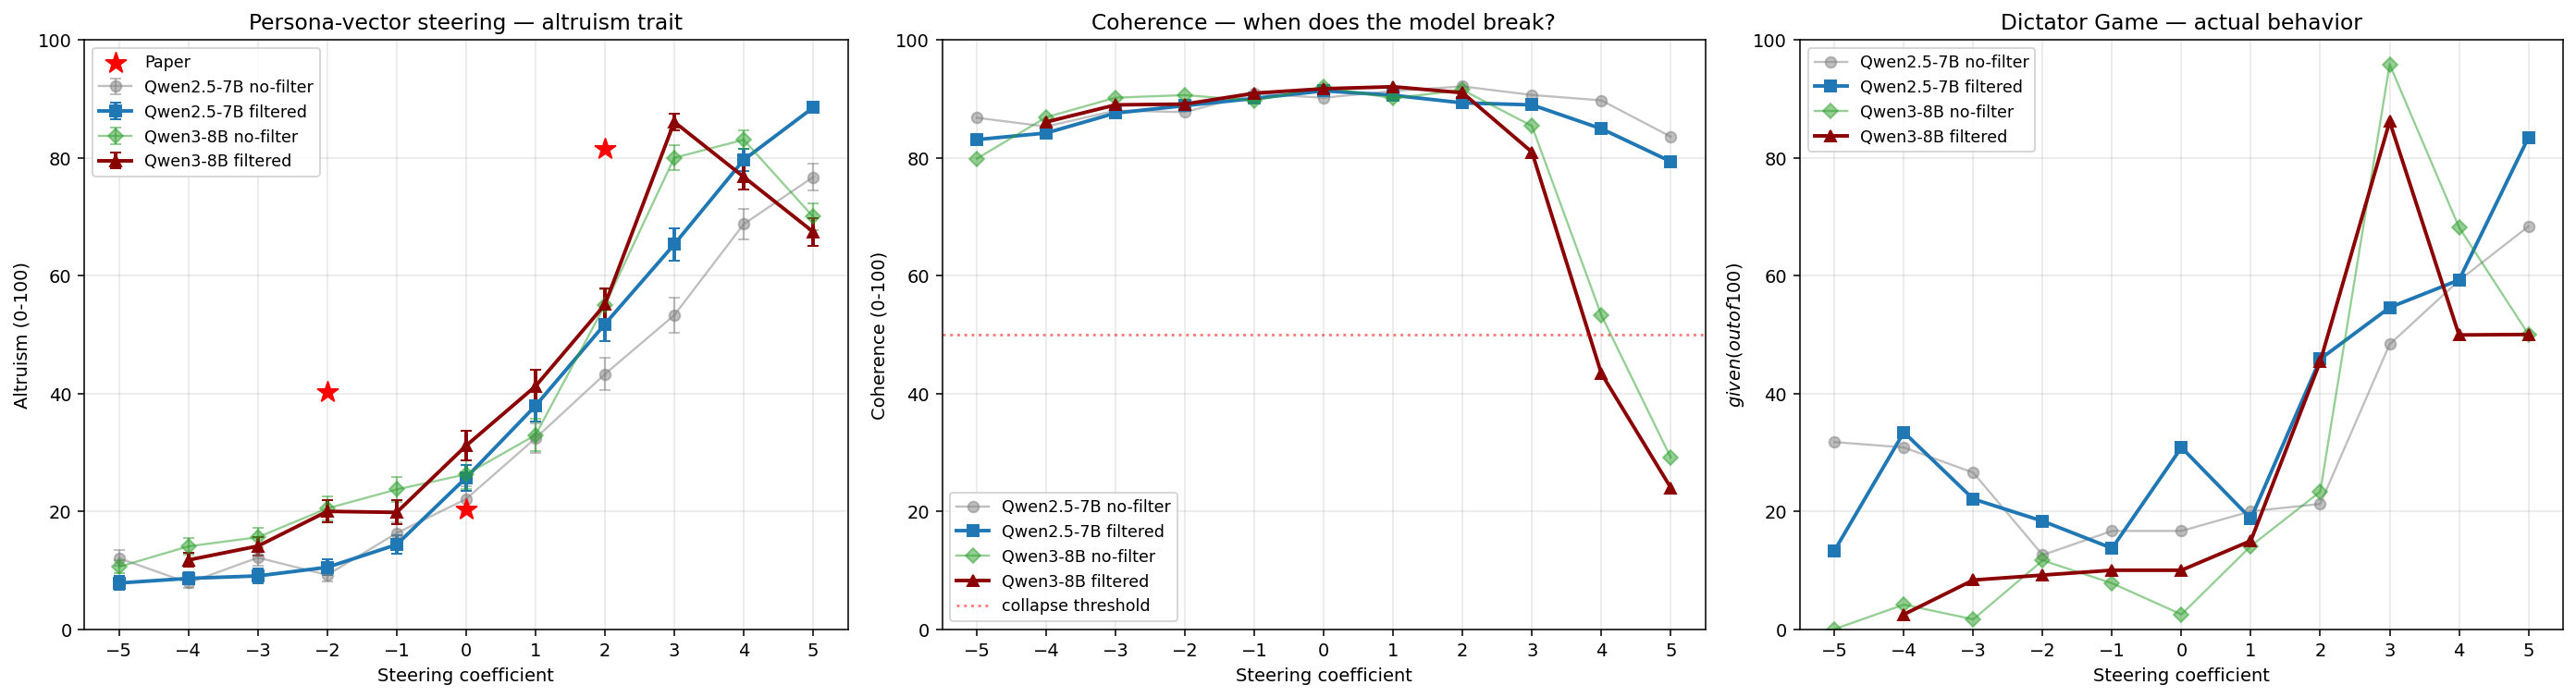
\includegraphics[width=\linewidth]{altruism_sweep_4cond.png}
\\{\scriptsize Altruism sweep: 4 условия.}
\end{columns}
\end{frame}

% --- 6. Фаза III геометрия (слитые 6+7) ---
\begin{frame}{Фаза III. $v_\text{RLHF}$ — это не черта характера}
\begin{columns}[T]
\column{0.52\linewidth}
$v_\text{RLHF}$ почти ортогонален altruism axis на трёх семействах (cos @ L20):
\begin{center}\footnotesize
\begin{tabular}{lccc}
\toprule
axis & Qwen2.5 & Qwen3 & Llama \\
\midrule
altruism & $-0.03$ & $+0.13$ & $+0.11$ \\
deliberation & $+0.20$ & $+0.24$ & $+0.27$ \\
safety & $+0.16$ & $+0.28$ & $+0.24$ \\
sycophancy & $-0.18$ & $+0.00$ & $-0.02$ \\
\bottomrule
\end{tabular}
\end{center}
{\footnotesize Altruism среди наименьших axes; доминирует elaboration / caution cluster. Семь axes вместе объясняют лишь 6–19\% направления (R$^2$ предварительный). Single-layer, на L20.}
\column{0.48\linewidth}
\centering
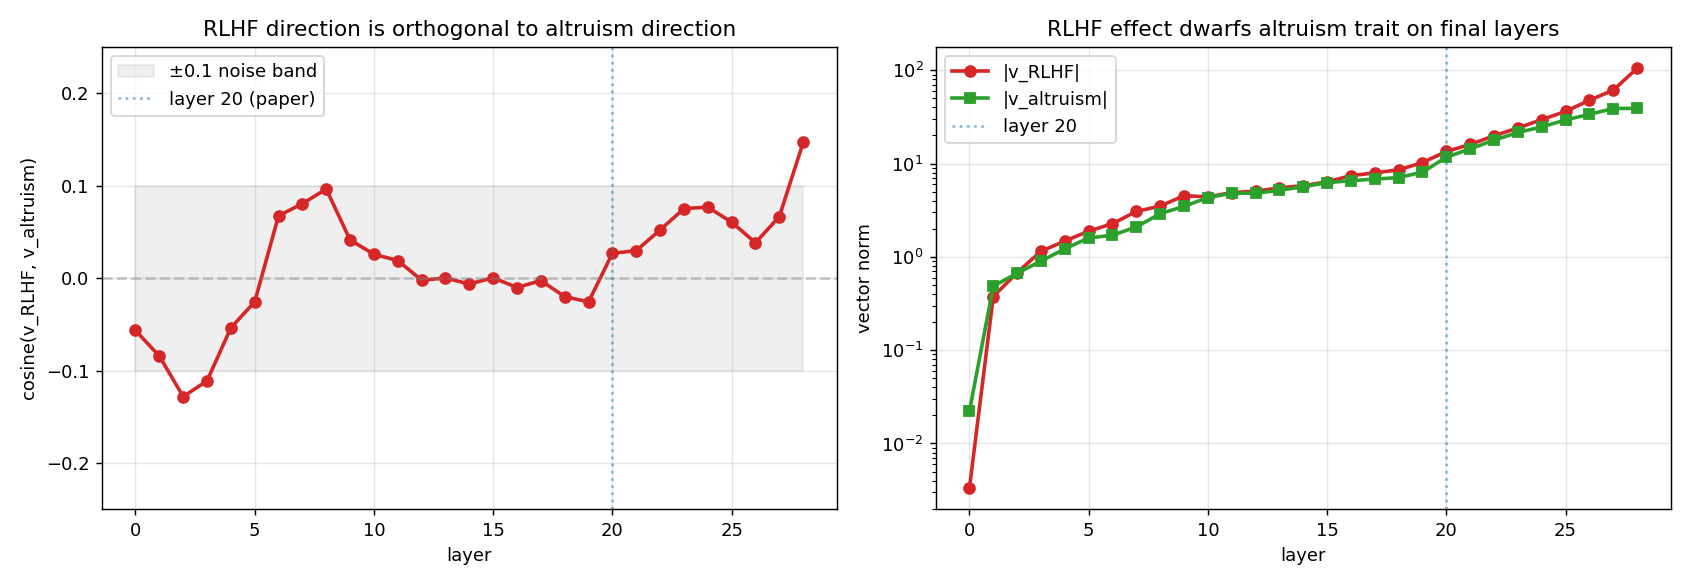
\includegraphics[width=\linewidth]{v_rlhf_vs_v_alt.png}
\\{\scriptsize Cos с altruism по слоям; нормы.}
\end{columns}
\end{frame}

% --- 7. Talk-vs-act (разбито на блоки) ---
\begin{frame}{Talk-vs-act: говорит $\neq$ делает}
\begin{block}{Говорит (вербальный балл судьи)}
\footnotesize Прирост после RLHF: Qwen2.5 $+5.5$ (p=.007), Qwen3 $+7.9$ (p=.002). Но ответы длиннее (156$\to$249, 235$\to$369 слов). Под контролем длины эффект исчезает: $-0.44$ / $+0.09$, n.s.
\end{block}
\begin{block}{Делает (реальные деньги в игре)}
\footnotesize На Qwen2.5 instruct отдаёт меньше базы (Dictator $-22.7$). Но это одна игра, один промпт, оценённый $\sim$30 раз: эффективное df $\approx 1$, демонстрация, а не популяционный вывод. На Qwen3 неубедительно: все доверительные интервалы пересекают ноль.
\end{block}
\end{frame}

% --- 8. v1/v2 ---
\begin{frame}{Два «направления RLHF» расходятся}
На одной модели (Qwen2.5) два принципиальных базиса экстракции дают почти ортогональные векторы: $\cos(v_1,v_2)=0.31$ (воспроизводимо, оба вектора в репозитории).
\begin{center}\footnotesize
\begin{tabular}{lcc}
\toprule
 & вербальный балл & деньги в Dictator \\
\midrule
v2 (response-pooled) & растёт с $+c$ & не двигаются ($\rho{=}{+}0.009$, p=0.95) \\
v1 (prompt-pooled) & плоско & снижается, но спутано с коллапсом coherence \\
\bottomrule
\end{tabular}
\end{center}
Это talk-vs-act в геометрии: axis «звучит щедрее» и axis «ведёт себя иначе» — разные. Act-side тонкий (один промпт), поэтому это интересное наблюдение, а не установленный механизм.
\end{frame}

% --- 9. BERT-валидация ---
\begin{frame}{Проверка: два length-робастных классификатора}
Те же ответы переоценены не-генеративными классификаторами (\texttt{bart-mnli}, \texttt{roberta-mnli}; «щедрый» vs «эгоистичный»). Прирост LLM-судьи не воспроизводит ни один (под контролем длины всё $\leq 0$):
\begin{center}\scriptsize
\begin{tabular}{lcccc}
\toprule
база$\to$instruct (под контр.\ длины) & LLM-судья & BERT-bart & BERT-roberta & Dictator \$ \\
\midrule
Qwen2.5 & $-0.4$ (n.s.) & $-11.2$ (p$<$.001) & $-5.0$ (p$=$.004) & $-22.7$ \\
Qwen3 & $+0.1$ (n.s.) & $-10.6$ (p$<$.001) & $-0.3$ (n.s.) & $-2.7$ \\
\bottomrule
\end{tabular}
\end{center}
{\scriptsize Каждое число — сдвиг base$\to$instruct: у судьи и BERT это балл альтруизма (шкала 0–100), у Dictator — реальная отдача (\$). Плюс $=$ instruct «добрее». Положителен только LLM-судья, и то незначимо.}\\[3pt]
{\footnotesize На Qwen2.5 сильный классификатор и реальные деньги сходятся: instruct менее щедр (roberta слабее, raw-разница около $-1.8$). Вывод: прирост судьи — артефакт многословия.}
\vspace{0.3em}

Обратный случай: \emph{steering} v2 даёт настоящий сдвиг содержания. Оба судьи видят рост, оба length-робастно (LLM $+3.79$, p=5e-4; BERT $+5.20$, p$<$1e-4), но денег это всё равно не двигает.
\end{frame}

% --- 10. Вывод (синтез, ссылка на тезис) ---
\begin{frame}{Что из этого следует}
Стандартный инструмент чтения «альтруизма от RLHF» — LLM-судья по свободному тексту — расходится с поведением сразу с нескольких сторон:
\begin{itemize}
  \item вербальный прирост держится на длине ответа, а не на содержании;
  \item геометрически $v_\text{RLHF}$ — это elaboration axis, а не altruism;
  \item steering двигает балл, но не реальную отдачу; а два базиса вектора расходятся.
\end{itemize}
\vspace{0.3em}
Предупреждение по методу: любая оценка ценностей или выравнивания через LLM-судью без контроля на длину может принять многословие за содержание.
\end{frame}

% --- 11. Отозванные выводы ---
\begin{frame}{Отозванные выводы}
Четыре первоначальных вывода не пережили проверку:
\begin{itemize}
  \item «Qwen3 после RLHF менее альтруистичен» — артефакт обрезки (86.5\% ответов резались на 250 токенах). На 1024 эффект разворачивается.
  \item «Qwen3 — рациональный отказник ($\$0$)» — классификатор нашёл 0\% явных отказов.
  \item «Subliminal SFT де-алайнит специфично» — контроль (учитель про сов) де-алайнит сильнее: эффект общий, не про altruism.
  \item «$v_\text{RLHF}$ снижает отдачу» — это были два разных вектора (v1/v2, cos 0.31); вывод превратился в диссоциацию.
\end{itemize}
Каждый отзыв исходит из контроля, классификатора или зафиксированного артефакта.
\end{frame}

% --- 12. Ограничения + future ---
\begin{frame}{Ограничения и что дальше}
\textbf{Ограничения.} Косинусы на одном слое (L20). Act-side — один промпт, df$\approx 1$; на Qwen3 неубедительно. R$^2$ предварительный. Судья сопряжён с длиной. Length-null зависит от фильтра coherence (без фильтра вербальный эффект частично выживает: длина И coherence).
\vspace{0.4em}

\textbf{Дальше.}
\begin{itemize}
  \item Расширить BERT-проверку (третий метод, эмбеддинги, ручная сверка).
  \item Мощная поведенческая батарея: $\geq 5$–10 формулировок каждой игры, промпт как случайный эффект — превратить демонстрацию в популяционный вывод.
  \item Выложить axis-векторы и скрипт, чтобы R$^2$ стал воспроизводимым.
\end{itemize}
\end{frame}

% --- 13. Закрытие (тезис как финал) ---
\begin{frame}{Одной фразой}
\begin{quote}
\large «RLHF делает модель добрее» по LLM-судье — в основном артефакт длины. Под контролем длины прирост исчезает, а length-робастный классификатор и реальные деньги на Qwen2.5 даже расходятся с судьёй.
\end{quote}
\vfill
\centering\footnotesize Репозиторий: \texttt{github.com/algorithm-pirogok/subliminal-persona-rlhf}
\end{frame}

\end{document}
